\subsection{Analysis of Surface Compression \label{Chapter 2: Quantitative Analysis of Surface Compression}}

\subsubsection{Simulation Dynamics}
This finite element approach can be extended to provide quantitative analysis of the indentation of surface features in AFM imaging. Of interest is the simulation of spherical and simple periodic structures. Within a natural setting, a hemisphere provides an analogy for various structures, and the deformation of a periodic structure provides a comparison for the analysis of DNA imaging. These structures were modelled as three-dimensional elastic parts in ABAQUS, with simulations focused on the compression produced from a single scan along the centre axis of the structures. Surfaces are assumed to be homogeneous and isotropic with a relative Young's modulus and Poisson ratio comparable to biomolecules as before. Indentations were simulated with a rigid, spherically capped conical indenter and "surface to surface" type contact. The contact was set as "hard", nonadhesive contact in the normal direction and "rough" Coulomb friction (non-slip) in the tangential direction. Boundary conditions fix the base of the structure, and vertical force and indentation data are mapped and sampled via reference points at the centre of the indenter. The simulations produced 2D force and indentation data over the central axis. The radial compression of spherical samples and the distortion in periodic structures are analysed as functions of the indentation force and the contact radius. The scan geometries are shown in Figure \ref{fig: Compression Simulation dynamics}, and the following section details the techniques used to analyse the data. Example scripts are viewable in Appendix \ref{Appendix: ABAQUS Script}.


\begin{figure}[H]
\centering
    \begin{subfigure}[t]{0.565\textwidth}
        \centering
        \caption{\label{fig: Compression Simulation dynamics-wave} }
        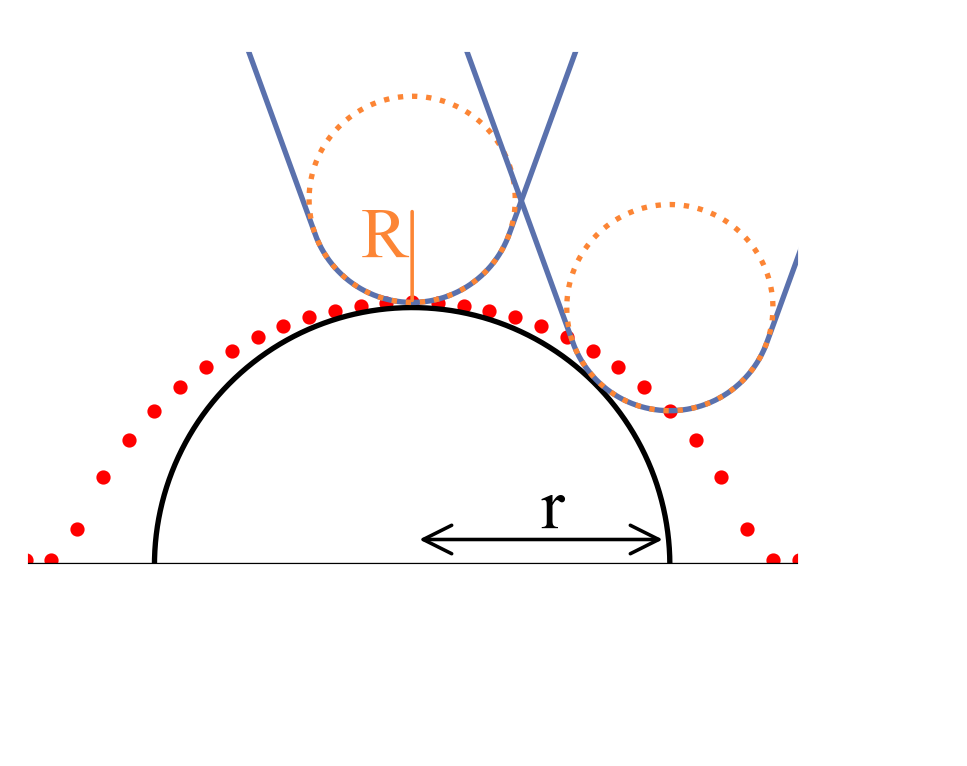
\includegraphics[trim = 0 45 0 0, clip, width=1\linewidth]{Figures/Hemisphere-SetUp.png}
    \end{subfigure}
    \hfill
    \begin{subfigure}[t]{0.415\textwidth}
        \centering
        \caption{\label{fig: Compression Simulation dynamics- wave} }
        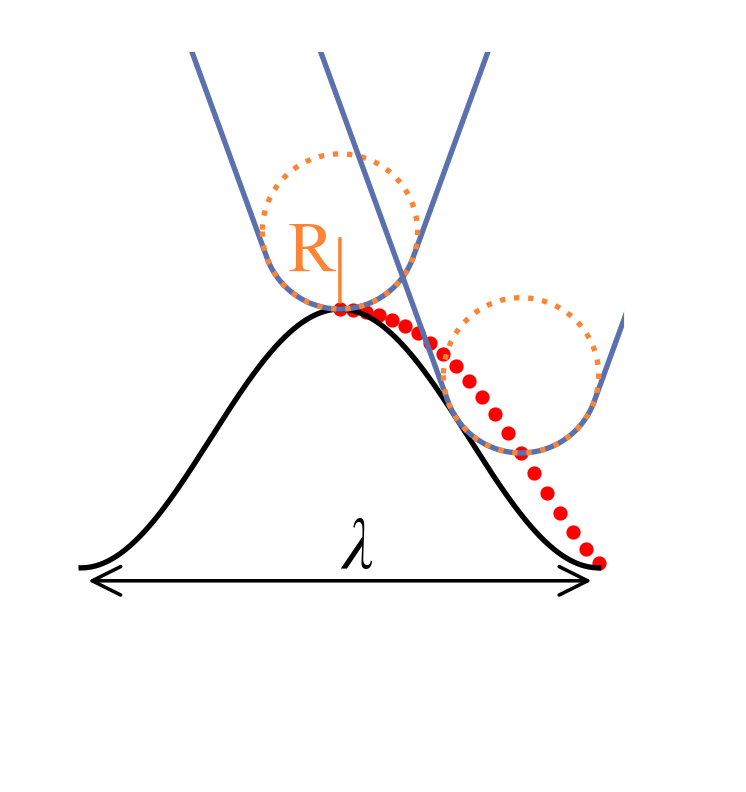
\includegraphics[trim = 0 45 0 0, clip, width=1\linewidth]{Figures/Wave-SetUp.png}
    \end{subfigure}
    
    \caption{\label{fig: Compression Simulation dynamics}(A) Geometry of scan along the central axis of a hemisphere. Three-dimensional geometry is produced by rotating the indenter and semi-circle around the central z-axis. The hemisphere is shown in black with a radius $r$. Indenter geometry is shown in blue with a circular tip of radius $R$ in orange. Red points indicate initial scan positions (Hard sphere contact points). (B) The geometry of the scan along the central axis of a plane wave structure for a half wavelength. Three-dimensional geometry is produced by rotating the indenter around the central z-axis and extruding the wave in the out-plane direction. Wave is shown in black with wavelength $\lambda$. Indenter geometry is shown in blue with a circular tip of radius $R$ in orange. Red points indicate initial scan positions (Hard sphere contact points). }
\end{figure}

\subsubsection{Heat Map and Force Contours}

A heat map of the force over the scan domain was produced by processing data from indentation simulations. The heat map are produced by iterating over the course-grained x and z coordinates of the scan and mapping the corresponding force at each position into a 2D grid of the scan domain. This provides a grid of the force across a cross-section of the surface. A mask is used to exclude positions with no indentation data. Similarly, the force contours are calculated by iterating over each x coordinate and evaluating the force. The code finds the index for the value equal to the reference force and stores the corresponding XZ position. If the maximum force is below the threshold, the code masks that value in the contour array. 


\subsubsection{Full Width Half Maxima}

Full-width half maximum (FWHM) measures the width of a peak in a spectrum at half of its maximum amplitude. FWHM characterise the resolution and peak shape of the contour. In Python, calculating the FWHM for the contour data is achieved by fitting a cubic spline to the contour data using the scipy.interpolate module. Once the spline is fitted, the FWHM can be calculated from the roots at half the maximum value. Finding the roots uses the UnivariateSpline.roots scipy function. This approach is advantageous because it provides a smooth representation of the data, which can help analyse noisy data sets.

\subsubsection{Fourier Analysis}

Fourier series express a periodic function as an infinite sum of sine and cosine waves, each modulated by an individual amplitude and frequency. Fitting data to a Fourier series allows for analysis of the spatial resolution of the contours produced. In Python, fitting data to a Fourier series is achieved using an explicit function for the series and scipy.optimise curve\_fit function. Data used to fit the series was extrapolated from a tight spline of the raw contour data. This is used to ensure the smoothness of the fit and avoid overfitting due to a reduced number of data points. The curve\_fit function returns the optimised coefficients and the covariance matrix. As the surface and contours are symmetric functions, Fourier analysis only requires the cosine terms given by, 

\begin{equation}
    F(x) \approx \sum^{\infty}_{n=0} A_{n} \cos\left( \frac{2\pi n t}{T}\right)
\end{equation}

\subsubsection{Volume Analysis}

Volume analysis provides a quantitative metric for compression and distortion at varying indentation forces. Volume was calculated from splines fitted to the force contours using the Scipy UnivariateSplines class. This class provides an integral method that can be used to calculate the definite integral of the spline over a specified interval. The integral method uses numerical integration techniques to approximate the area under the curve, which can then be interpreted as the volume.

\subsubsection{Youngs Modulus}

The variation of fitted Young's Modulus over the scan positions illustrates the perceived elastic response of the surface. We use the same procedure used for contact models to fit the Hertz model in Python. Using the Scipy curve\_fit function, the Hertz model is fitted for the indentation data at each scan position. Young's modulus is used as the fitting parameter—this returns the variation of fitted Young's modulus over the scan positions.